

\chapter{The Item/System Problem}


When accounts of social-cultural transmission are explicit about the 
causal processes involved, we see that they often take cultural \textit{
items}---rather than systems---as their unit of analysis. This works well 
but it is awkward because we know that cultural items don't exist in 
isolation. We can only make sense of cultural items in the context of a 
\textit{system} or field of cultural meaning. 



Higher-level systems like languages and cultures show such a coherence 
of structure that we are seduced into thinking of them as organisms with 
bodies (see classic statements of philologists von der Gabelentz 1891 
and Meillet 1926, 16). Compare this to the situation in vertebrate 
biology. Genes are distinct entities yet they \textquoteleft caucus' and \textquoteleft form 
alliances' thanks to the bodies and body plans in which they are 
instantiated (Gould 1977, cited in; Dawkins 1982, 117). The difference 
is that vertebrates actually do have bodies while cultural systems 
do not. 



The pieces of a cultural system aren't held together by physical 
attachment to a shared material whole. So this is our puzzle. If 
languages and other cultural systems \textquoteleft hang together', what is the 
binding force? If cultural transmission involves causal processes that 
apply only to small parts of the larger whole, what explains the 
coherence of that larger whole? This is the item/system problem.



Here is the solution. The ideas of \textquoteleft cultural item' 
and \textquoteleft cultural system' are reconciled by something that they have in 
common: Neither idea exists without the simpler idea of a \textit{
functional relation}. 



A word---\textit{kangaroo}, for example---is easily thought of as a 
distinct cultural item. One can cite it or borrow it without having to 
also cite or borrow the language system that it comes from. But the word 
cannot be defined or understood---nor can it exist---except in terms of its 
functional relation to other things, things like the words it co-occurs 
with, the conversations in which it is used for referring to kangaroos, 
and so on. 



Ditto for technology. A spoke can be designed, named, bought, and sold, 
but as a cultural item, a spoke doesn't make sense without a wheel. And 
while a wheel is a whole when thought of with reference to a spoke, it 
is a \textit{part} when thought of with reference to a vehicle, and so 
on. 



In sum: An item doesn't make sense without functional relations to other 
things, just as a system doesn't make sense without the functional 
relations it incorporates. Functional relations are the interface that 
joins items and systems together, and we can look to them for a solution 
to the item/system problem.

\section{A transmission criterion}


In the causal ontology of culture, there is a \textit{transmission 
criterion}. Since-by definition-social facts cease to exist if 
individual people stop behaving as if they exist, and since social facts 
endure with relative stability beyond individual people's lifetimes, 
then social facts must be transmitted among individuals in human 
populations in order to (i) exist and (ii) endure with relative 
stability. Transmission is a necessary part of what makes culture and 
language the way they are. 



A causal account of culture depends, then, in part at least, on an 
account of how culture is transmitted within human groups and across 
generations. Much is known about how \textit{items} are transmitted 
(Rogers 2003, inter alia), but macro-level cultural systems cannot be 
transmitted in the same way. 



Do we need two separate accounts of transmission, one for items, one for 
systems? I am going to argue that we can derive system transmission from 
item transmission, on the condition that we have a more accurate 
definition of items. We can define items not as cultural things but as 
cultural things with functional relations to other cultural things. 
Cultural items are specified for-and advertise-their relations to the 
contexts into which they fit (where, it must be said, this \textquoteleft fit' can be 
quickly and easily re-tooled). As Kockelman (2013, 19) writes: \textquoteleft there 
are no isolated environments and organisms, there are only \textit{
envorganisms}.' 

\section{Systems}


To understand what a cultural system is, first consider the notion of 
item. A cultural item is any seemingly detachable conceived entity such 
as a piece of technology, a technique, a way of saying something, a 
value. An item can be readily defined and labeled, and can be learned 
and borrowed from one human group into another (though typically with 
some transformation of significance in the new context). Object-like 
things such as tomahawks might be prototypical items, but the notion of 
item intended here also includes train tracks, AC current, and 
mother-in-law avoidance. 



By contrast, a cultural system is a coherent set of such items, each 
item related to the others. A system has a higher-level holism that goes 
beyond the sum of the parts, in the sense that the full meaning of any 
individual cultural item is determined in the context of a set of 
relations into which it fits, and within which it serves a function. 
Often, we cannot observe the system directly or in one go, as for 
example in the case of a language or a telecommunications 
infrastructure, though this is sometimes made virtually possible by 
means of \textit{signs of} these systems that scale them down in such 
a way as to produce a \textquoteleft tangible expression', as Durkheim put it (1912, 
208), of the more diffuse phenomenon. 



A book can contain a grammatical description of a language, or a diagram 
can portray the elements of a telecommunications system in miniature. In 
these cases a representation of the system is created and/or inferred 
from an aggregate of encounters with context-situated items. These 
itemized emblems have different affordances from the real systems they 
represent, and they have different collateral effects as a result of 
their form. A grammar book, for example, promotes the idea that a 
language is a finite, bounded thing; in short, an item. 



As we now turn to examine systems in more detail let me emphasize in 
advance that neither items nor systems can be understood, nor indeed can 
they exist, without the \textit{relations }that are inherent in both. 
Relations are definitive for both items and systems. For an item, 
relations define its \textit{functions}. For a system, relations 
define its \textit{structure}.



A system should have at least these three properties: (1) it can readily 
be construed as a thing with multiple inter-related parts; (2) effects 
on one part should have effects on other parts; and (3) the parts should 
together form a whole in the sense that they are more closely related to 
each other than they are to other things, outside the system. 



Good examples are biological or ecological systems. In a food chain, 
populations of different species are inter-related, where changes in the 
frequency or behavior of one species will affect the frequency or 
behavior of others. While each species in the ecosystem will ultimately 
be connected to entities outside the focal food chain system, the 
integration \textit{within }the system is greater. 



Clearly, on all three counts, whether or not we are looking at a system 
is ultimately a matter of construal (see fn. 10, above). To say that a 
set of entities forms a system is partly just a way of looking at those 
entities. 


\textit{note:} \textquoteleft There is evidence that grammatical change is not always limited to the language acquisition process. The grammar of an adult can change.' (H\&C:49)
'[T]he grammar of an adult is best viewed, not as an inflexible completed object, but as an adaptable, constantly growing set of generalisations.' (H\&C:49)


\section{Relations between relations as a seed for systems}


Culture and language hinge on shared meaning, and so our focus in this 
chapter is on \textit{semiotic }systems. The idea of a semiotic system 
is well illustrated in Darwin's account of the expression of emotion in 
animals. Darwin introduces a principle of \textit{functional connection 
}between a sign and what it stands for. 



In his example, the visible features of a dog in a \textquoteleft hostile frame of 
mind'-upright, stiff posture, head forward, tail erect and rigid, 
bristling hairs, ears forward, fixed stare-are intelligible because they 
recognizably \textquoteleft follow from the dog's intention to attack'. Figure 1 is 
Darwin's illustration:


\begin{figure}[h!]
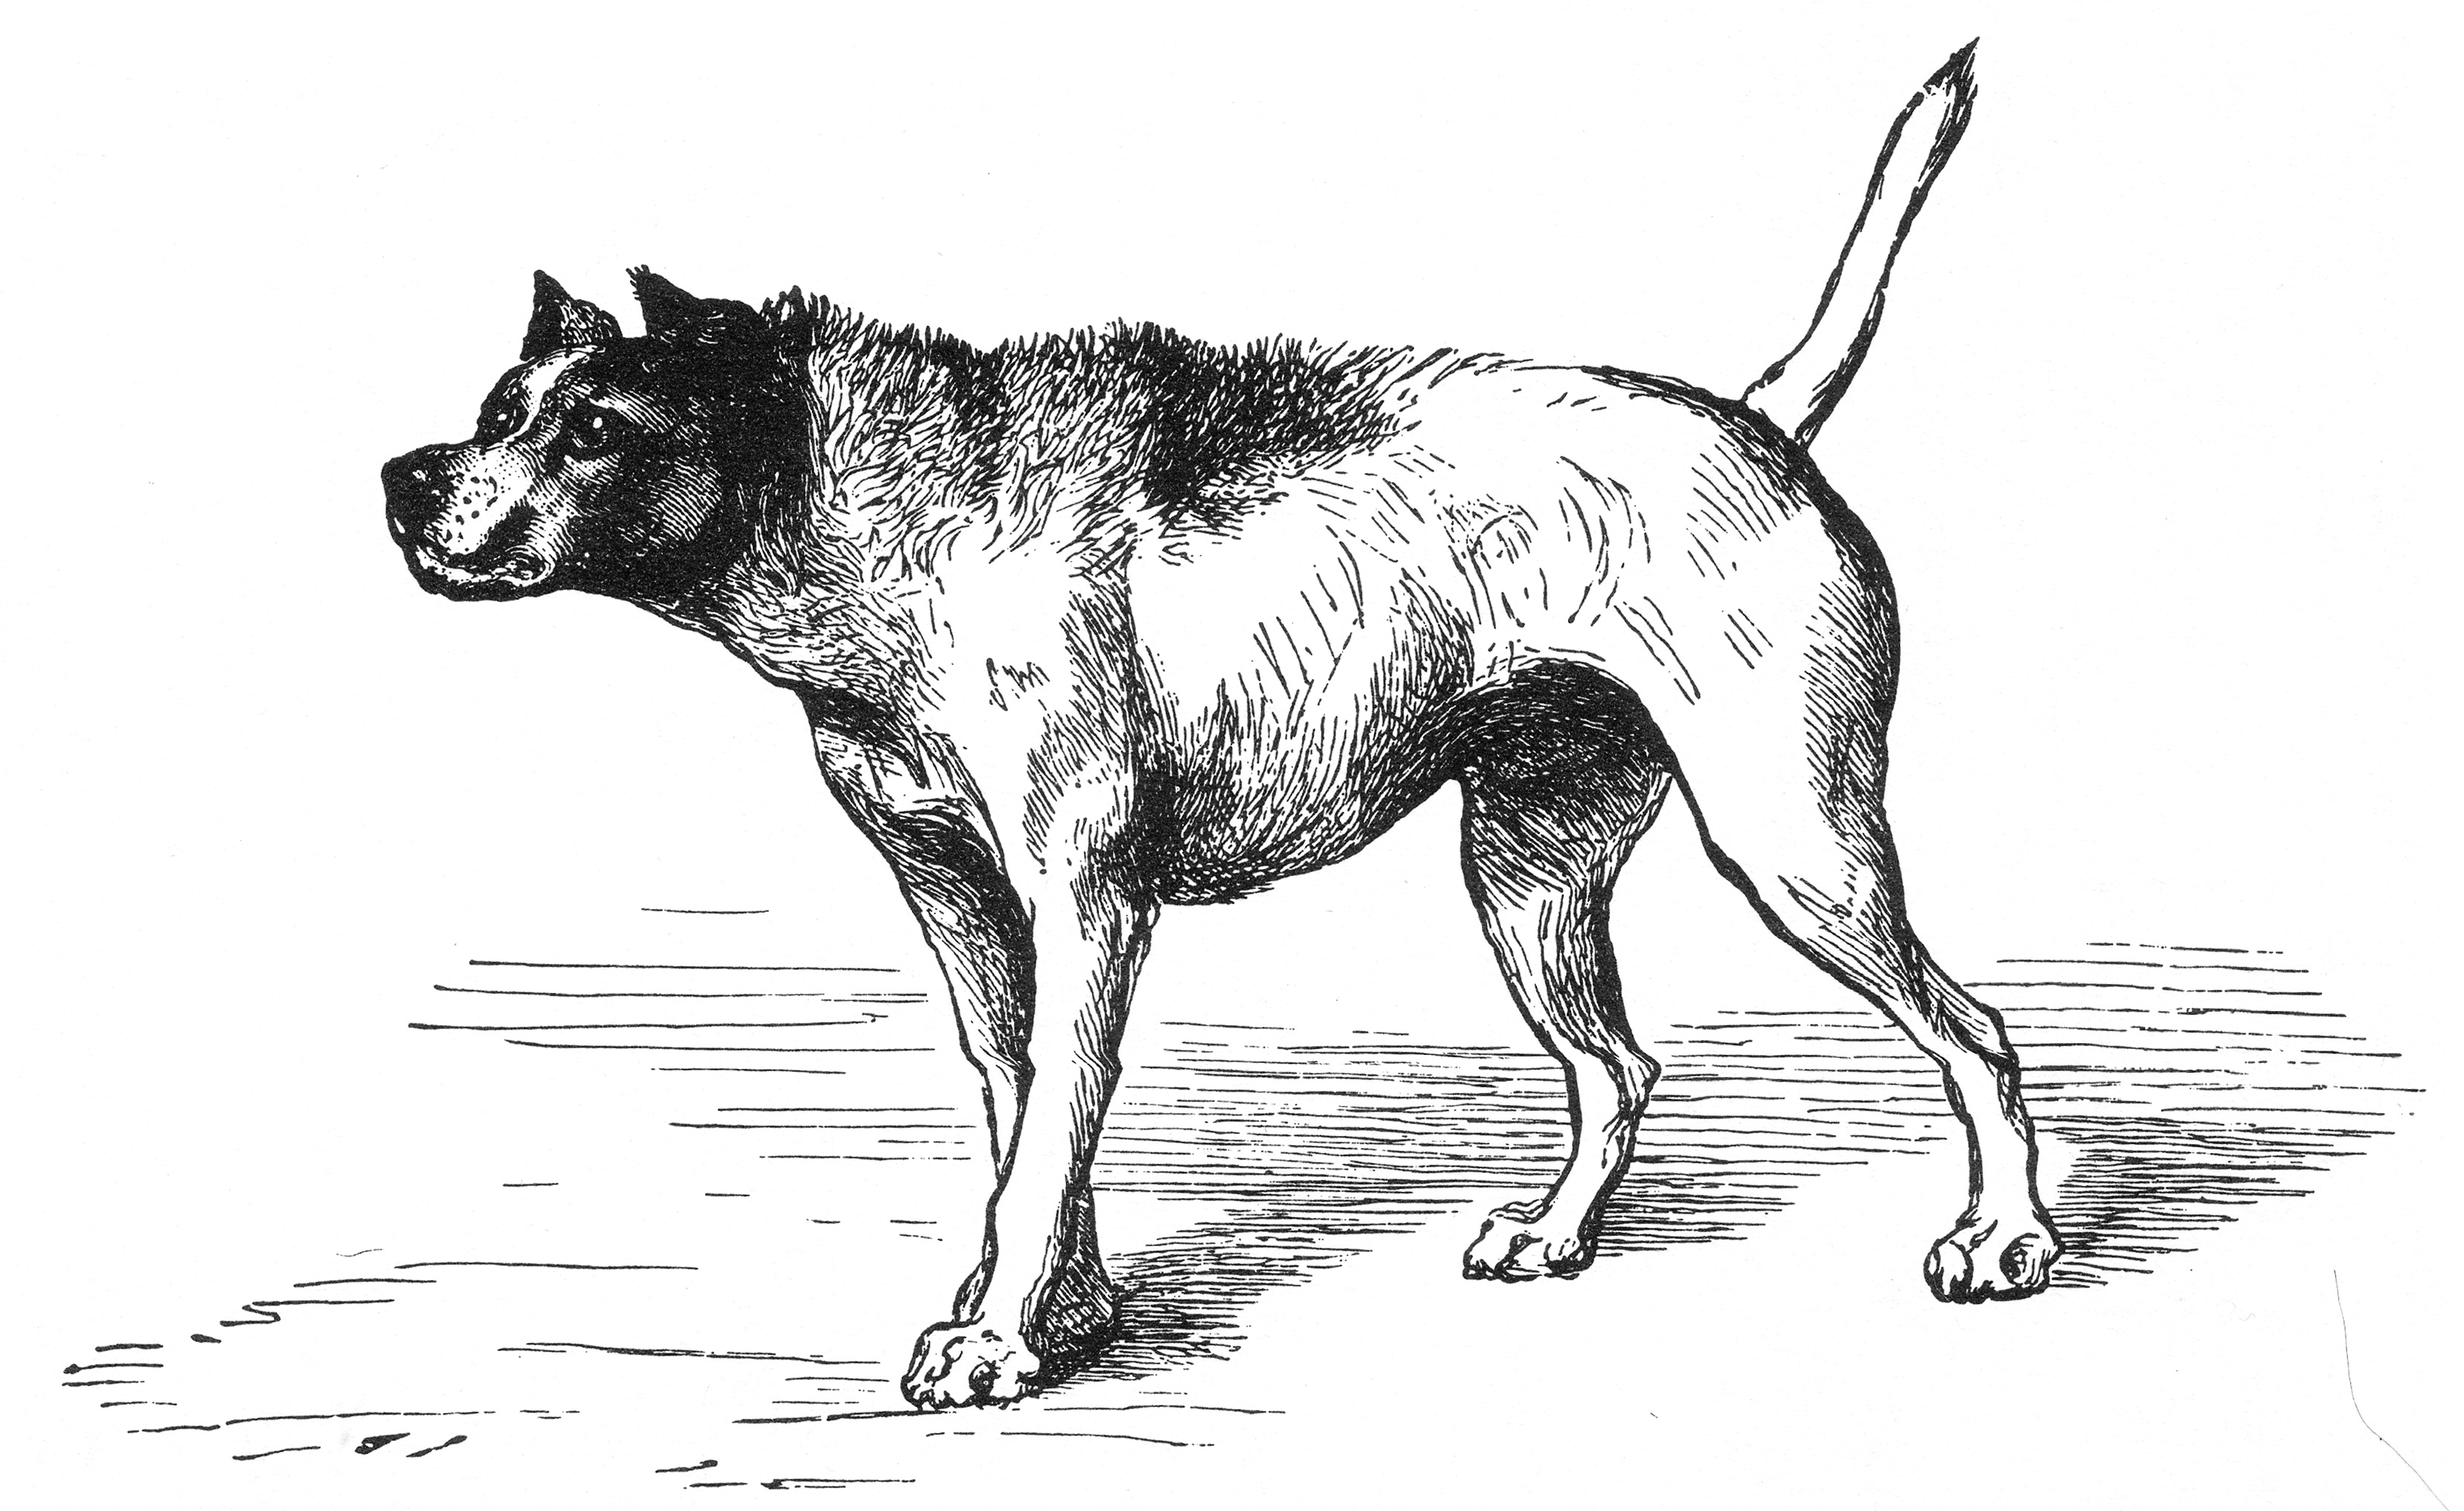
\includegraphics[width=0.90\textwidth,keepaspectratio]{figures/Fig01}
\caption{Darwin's illustration of a dog in hostile frame of mind 
(Figure 5 from \textit{The Expression of the Emotions in Man and 
Animals})}
\end{figure}



These behaviors are functionally connected to the aggressive attitude, 
and thus come to signal it. This can be illustrated as in Figure 2:

\begin{figure}[h!]
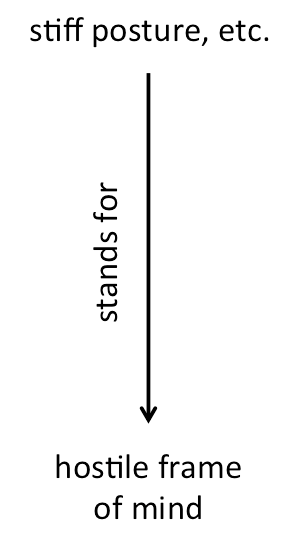
\includegraphics[width=0.30\textwidth,height=\textheight,keepaspectratio]{figures/Fig02}
\caption{A \textquoteleft functional', indexical association between observable 
behaviour and frame of mind (after Darwin).}
\end{figure}


This is only a first step toward establishing a semiotic system. Figure 
2 shows a relatively simple relation, a positive association between an 
observable behavior and a frame of mind, from which one might produce a 
range of relevant interpretants (e.g., running away, grabbing a big 
stick, etc.). 



From this, Darwin argues for a second signalling principle, called 
\textit{antithesis}. By exploiting the already-established semiotic 
relation shown in Figure 2, the dog can express the \textit{opposite} 
of aggression by \textquoteleft reversing his whole bearing', that is, doing the 
'opposite' of what one would do when aggressive. Thus, when approaching 
his master in an affectionate attitude, visible behaviors include body 
down, \textquoteleft flexuous movements', head up, lowered wagging tail, smooth hair, 
ears loosely back, loose hanging lips, eyes relaxed. Figure 3 is 
Darwin's illustration:


\begin{figure}[h!]
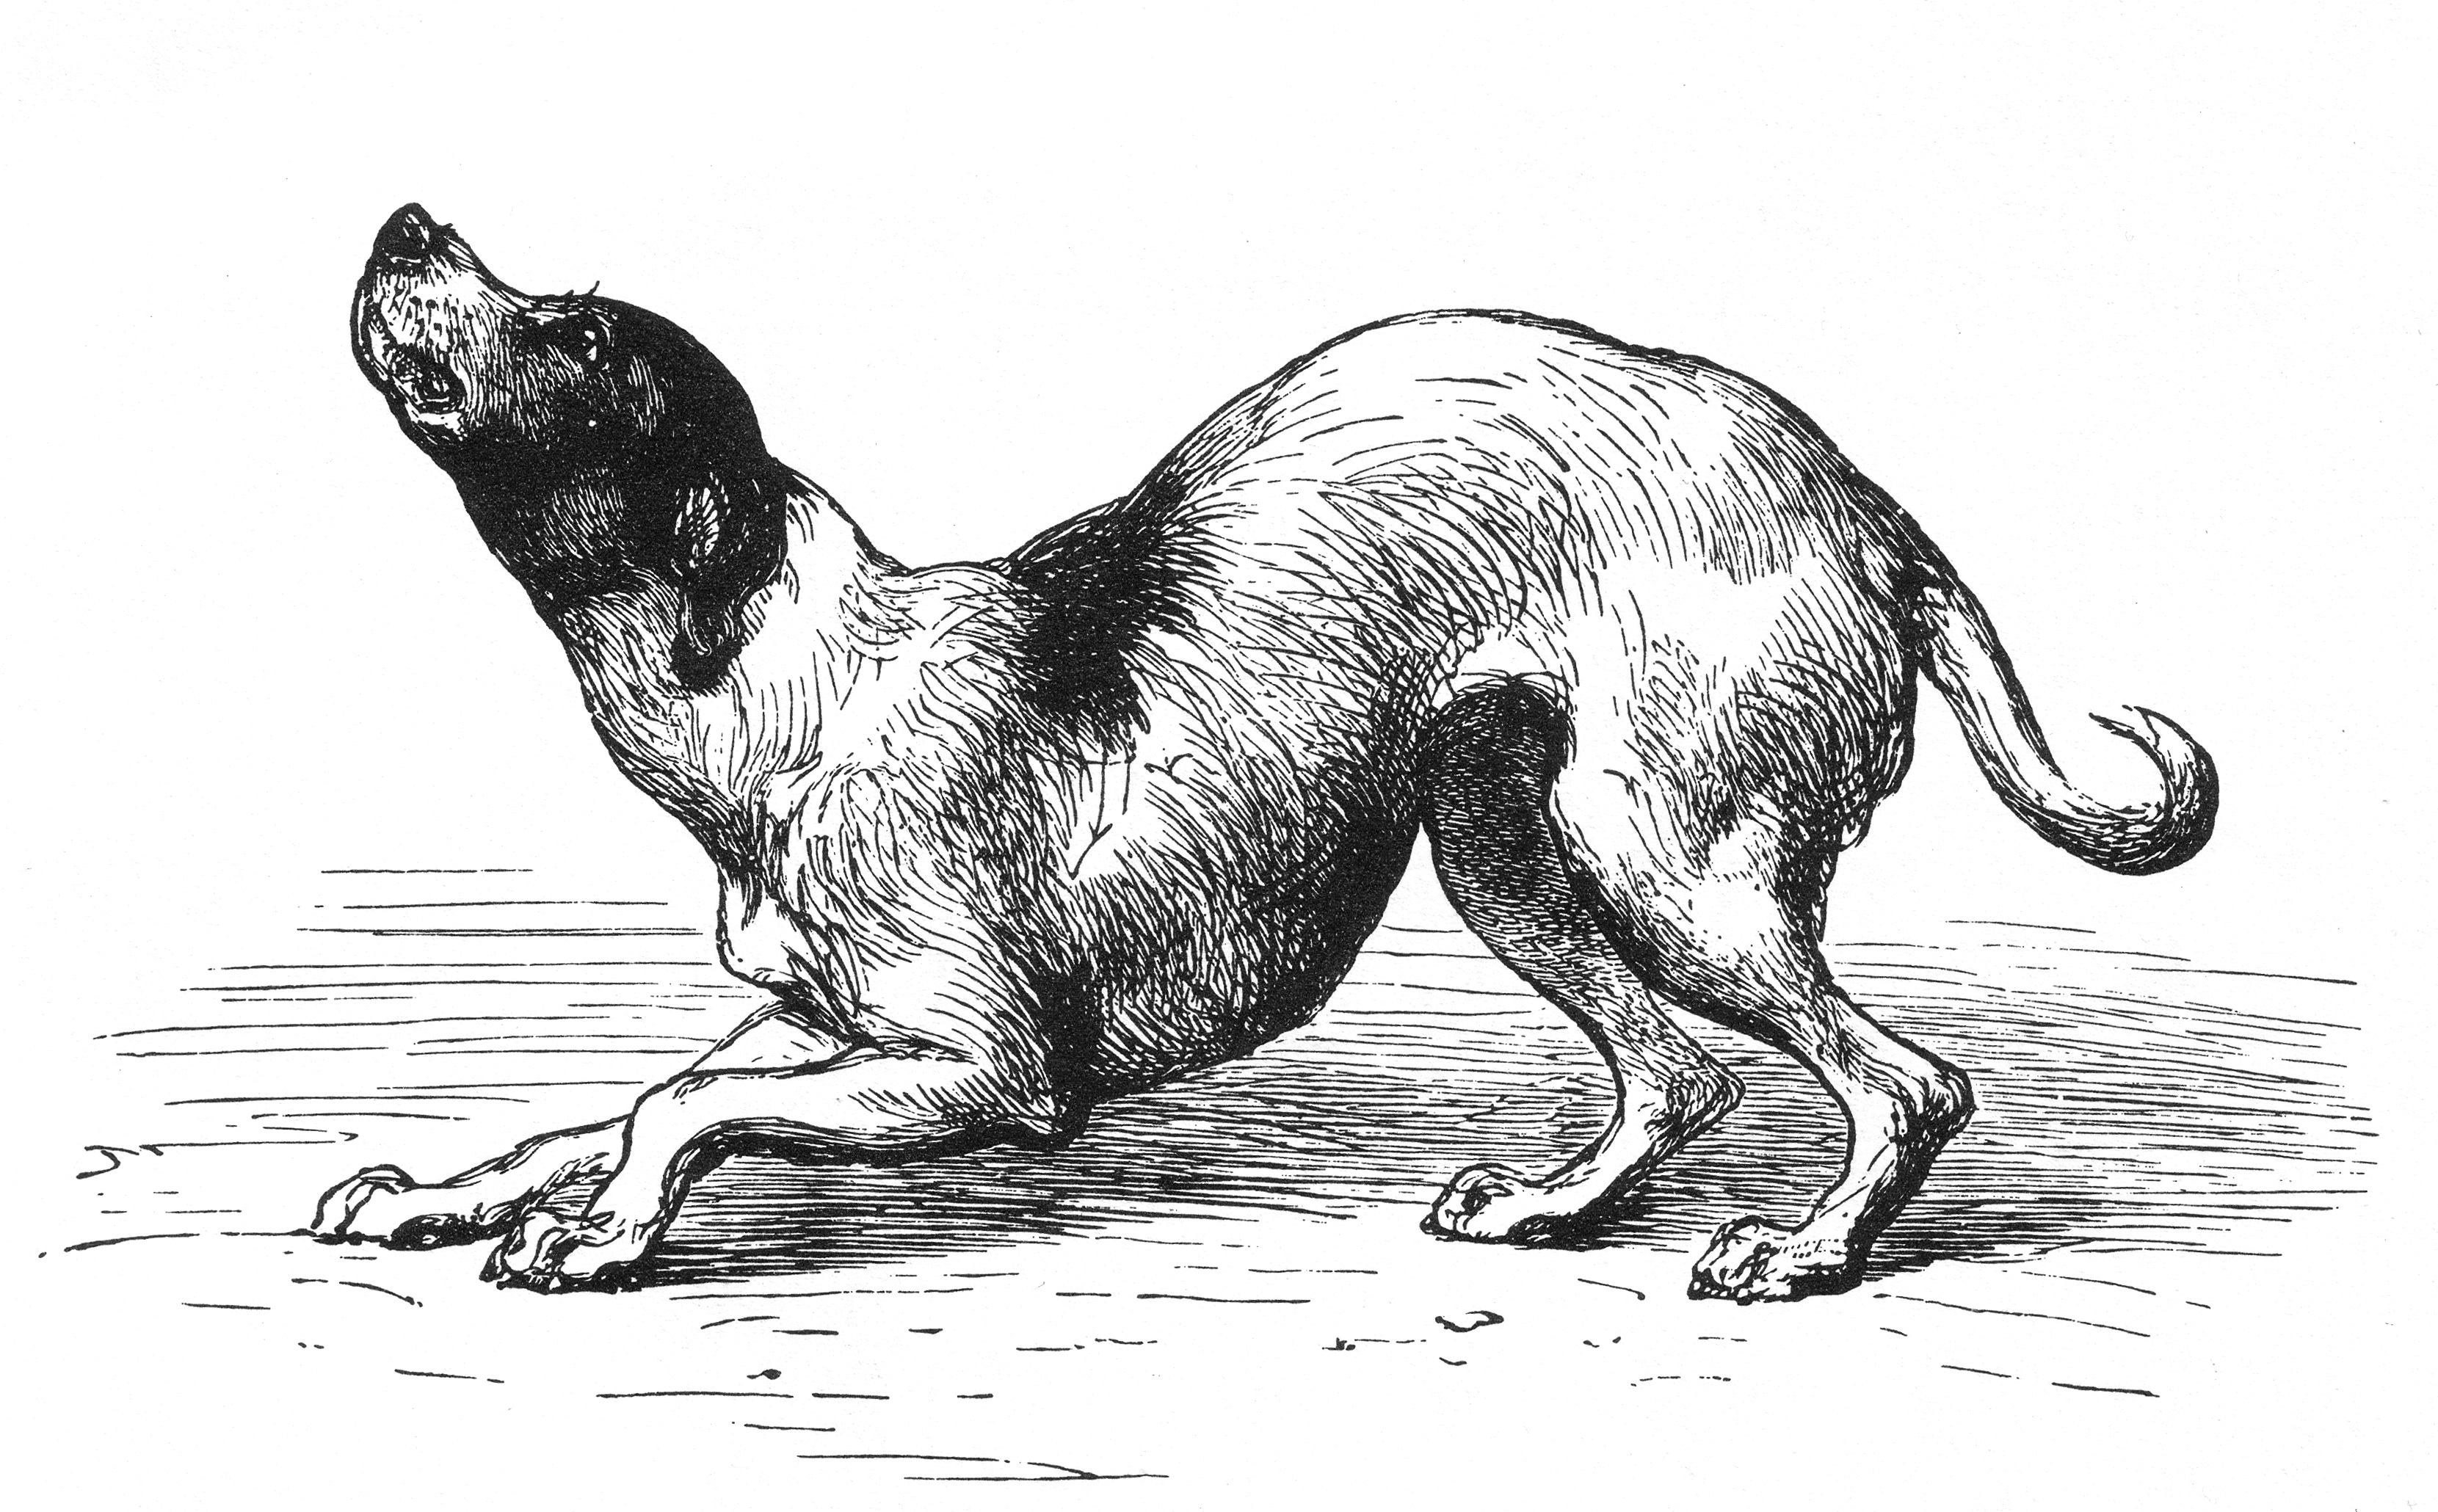
\includegraphics[width=0.9\textwidth,keepaspectratio]{figures/Fig03}
\caption{Darwin's illustration of a dog in an affectionate attitude 
(Figure 6 from \textit{The Expression of the Emotions in Man and 
Animals})}
\end{figure}




'None of $[$these$]$ movements' wrote Darwin, \textquoteleft so clearly expressive of 
affection, is of the least direct service to the animal. They are 
explicable, as far as I can see, solely from being in complete 
opposition to the attitude and movements which are assumed when a dog 
intends to fight, and which consequently are expressive of anger.' 
(Darwin 1872, 15-16). This can be illustrated as shown in Figure 4:


\begin{figure}[h!]
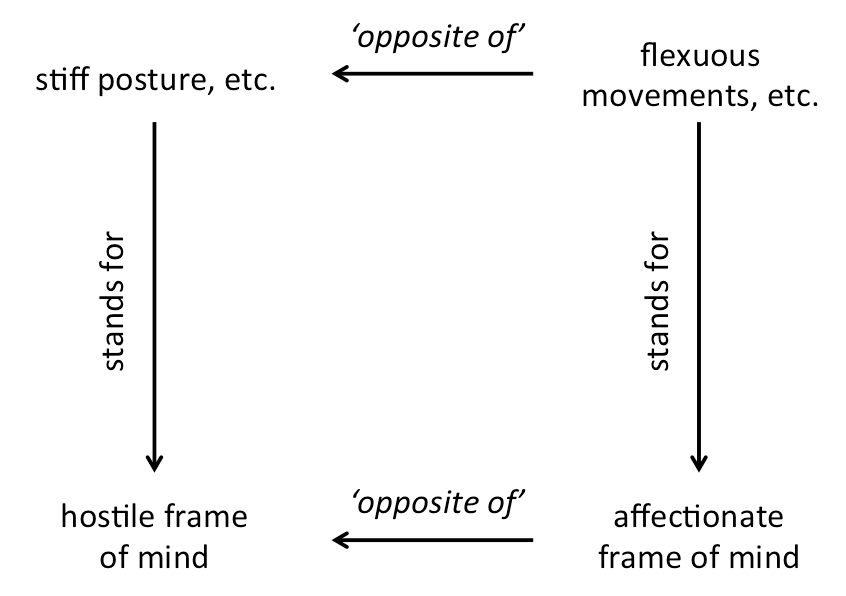
\includegraphics[width=0.9\textwidth,keepaspectratio]{figures/Fig04}
\caption{A secondary indexical association between observable behavior 
and frame of mind (at right), deriving its meaning only in connection 
with the established relation illustrated in Figure 2 (and incorporated 
at left of this Figure), assuming the interpreter's knowledge of a 
limited range of possible bodily behaviors, on the one hand, and a 
limited set of frames of mind, on the other (after Darwin).}
\end{figure}

As depicted in Figure 4, antithesis is a secondary relation. As Darwin 
pointed out, it depends on the interpreter's already-established 
recognition of a specific functional relation. But there is something 
more that it depends on, something crucial to the idea of a semiotic 
system. It is entailed by the term \textquoteleft opposite'. 



To recognize that a certain behavior is \textit{the opposite} of some 
other behavior, as opposed to simply \textit{not} that other behavior, 
one must be able to consider alternative possibilities within a 
restricted set. Flexuous movements can be recognized as the opposite of 
the aggression-signaling behavior only when one knows, or can predict, a 
limited range of postures that a dog can make. And for this to work in 
the way depicted in Figure 4, one must also understand that there is a 
limited set of relevant frames of mind that the dog may have, such that 
aggressive is at one end and affectionate at the other. 



This basic type of semiotic system arising from Darwin's principle of 
antithesis sets up relations-between-relations (Kockelman 2013, 12ff) by 
presupposing the interpreter's access to other systems such as body 
posture and emotional state, with some sense of their component elements 
and the logical-causal relations between them (e.g., that if one is 
being affectionate one is necessarily not being aggressive, or that if 
one's body is stiff it cannot also be flexuous). 



Central to the notion of functional relation to context that I have 
argued for so far are the concepts of \textit{incorporation }and 
\textit{contextualization}. These are defined in semiotic terms by 
Kockelman (2006, 29), as follows:



\textit{Incorporation}

For any two semiotic processes, A and B, A will be said to incorporate B 
(and hence be an interpretant of it) if the sign of B relates to the 
sign of A as part-to-whole, and the object of B relates to the object of 
A as means-to-ends. For example, in the case of instruments (semiotic 
processes whose sign is an artificed entity and whose object is a 
function), a wheel incorporates a spoke.



\textit{Contextualization}

For any two semiotic processes, A and B, A will be said to contextualize 
B, if A is required to interpret B, or at least assists in interpreting 
B. For example, a hammer contextualizes a nail. And a sword 
contextualizes a sheath. That is, nails make no sense without the 
existence of hammers; and sheaths make no sense without the existence of 
swords.



Incorporation and contextualization are widely applicable concepts in 
defining functional relations. They hold, for example, for the relations 
between a verb and a clause, a handle and a knife, a marriage rule and a 
kinship system. They are the basis of combinatoric rules, and as such 
they ultimately account for grammar in the complete sense (assuming a 
semantically-based approach to grammar; cf. Langacker 1987; Wierzbicka 
1988; Croft 2000, inter alia). 



\section{More complex systems: linguistic grammars}


The basic relations-between-relations structure depicted in Figure 4, 
combined with the functionally recursive embedding relation of 
incorporation is the essence of the kinds of semiotic systems that 
characterize the grammatical organization of any natural language 
(Saussure 1916; see Dixon, 2014; Bickel, 2014). 



All languages have systems of form classes, by which the thousands of 
words and other meaningful elements that one must learn in order to 
speak the language can be grouped and categorized in terms of their 
distribution relative to each other. Thus, we find open classes of 
content words like nouns and verbs versus closed classes of function 
words like prepositions (e.g., in English) and case-marking affixes 
(e.g., in Finnish). 



Then there are constructional systems defined by combinatoric 
principles. As an example consider the system for describing motion 
events in Lao (Enfield 2007, 387ff), consisting of three consecutive 
slots in a multi-verb construction, where each slot may be filled with a 
verb from three distinct sets, the first referring to the manner of 
motion (this is an open set), the second referring to the path of motion 
(from a set of 10 verbs), and the third referring to the 
direction of motion in relation to the deictic centre (from a closed set 
of 3 verbs):

\newpage
\ea Lao directional verb system

\begin{table}[htbp]
 % \centering
      \begin{tabular}{lll}
  
    SLOT 1 & SLOT 2 & SLOT 3 \\

    Verb of manner & Verb of path & Verb of direction \\
    open class & closed (n=10) & closed (n=3) \\
    \textit{lèèn1} ‘run’ & \textit{khùn5} ‘ascend’ & \textit{paj3} ‘go’ \\
    \textit{ñaang1} ‘walk’ & \textit{long2} ‘descend’ & \textit{mùa2} ‘return’ \\
    \textit{king4} ‘roll’ & \textit{khaw5} ‘enter’ & \textit{maa2} ‘come’ \\
    \textit{lùan1} ‘slide’ & \textit{qòòk5} ‘exit’ &  \\
    \textit{tên4} ‘jump’ & \textit{khaam5} ‘cross.over’ &  \\
    \textit{lòòj2} ‘float’ & \textit{lòòt4} ‘cross.under’ &  \\
    \textit{khii1} ‘ride’ & \textit{taam3} ‘follow’ &  \\
    \textit{khaan2} ‘crawl’ & \textit{phaan1} ‘pass’ &  \\
    \textit{taj1} ‘creep’ & \textit{liap4} ‘go along edge’ &  \\
    \textit{com1} ‘sink’ & \textit{qòòm4} ‘go around’ &  \\
    \textit{doot4} ‘leap’ &       &  \\
    etc.  &       &  \\
   
    \end{tabular}%
  \label{tab:addlabel}%
\end{table}%

 \z



With this system, Lao speakers can generate utterances like the 
following:

\ea
\gll khaan2 qook5 paj3 \\
     crawl  exit  go\\
\glt \textquoteleft (S/he/it) crawled out/away.'
\z

\ea
\gll khaan2 qook5 paj3 \\
     crawl  exit  go \\
\glt \textquoteleft (S/he/it) crawled out/away.'
\z

\ea
\gll doot5 long2 maa2 \\
     leap descend come \\
\glt \textquoteleft (S/he/it) leapt down here.'
\z

\ea
\gll looj2 phaan1 mua2 \\
     float pass return \\
\glt \textquoteleft (S/he/it) floated back past.'
\z


This little linguistic sub-system illustrates the fundamental 
intersection between a syntagmatic axis (the left-to-right axis along 
which separate elements combine) and a paradigmatic axis (the slots 
which may be filled by alternative members of a set, with contrast 
effects between possible values not unlike the way a dog's stiff posture 
is opposed to a flexuous posture). 



Sub-systems in language interact with each other and show dependencies 
in higher-level systems such as those defined in comprehensive 
grammatical descriptions. Aikhenvald and Dixon (1998) describe 
dependencies among grammatical sub-systems. They show, for example, that 
the system of polarity (positive versus negative in relation to a 
predicate or clause) constrains many other systems in the grammars of 
the world's languages. 



In Estonian, there is a system in which person and number are 
distinguished by morphological marking on the verbs, but these 
distinctions are only realised in positive polarity. The distinctions 
are lost in the negative:



(5) \ \ \ \ Verb \textquoteleft to be' in Estonian



\begin{table}[h]
\centering
\begin{tabular}{|l|l|l|}
\hline
POSITIVE & & NEGATIVE \\
\hline
\textit{olen} (\textsc{1sg)}, \textit{oleme} (\textsc{1pl}) 
& & \\
\hline
\textit{oled} (\textsc{2sg)}, \textit{olete }(\textsc{2pl)} & 
& \textit{ei ole} (1/2/3\textsc{sg/pl}) \\
\hline
\textit{on} (\textsc{3sg/pl}) & & \\
\hline
\end{tabular}
\end{table}


Aikhenvald and Dixon (1998) present a cross-linguistic hierarchy of such 
dependencies between sub-systems. Such inter-connectedness between 
paradigm sets and combinatoric rules, and between sub-systems in a 
language, is evidence for the higher-level system properties of 
linguistic behavior. 



What follows from these facts about linguistic systems is that we cannot 
view any piece of language as a mere item. \textquoteleft A living language is not 
just a collection of autonomous parts', say Donegan and Stampe (1983, 
1). A language is \textquoteleft a harmonious and self-contained whole, massively 
resistant to change from without, which evolves according to an 
enigmatic, but unmistakably real, inner plan' (Donegan and Stampe 1983, 
1). 



They illustrate their point in explaining how it is that the languages 
of two sides of the Austroasiatic language family-Munda and 
Mon-Khmer-show a list of typological distinctions that are \textquoteleft exactly 
opposite at every level of structure' (Donegan and Stampe 2002, 111) 
despite being demonstrably descended from the same Proto language. They 
argue that when speakers of Munda innovated a new prosodic profile, they 
were tampering with something that \textquoteleft pervades every level of language 
structure' (1983, 14). A simple change from iambic to trochaic stress 
had systemic knock-on effects that changed the entire morphosyntactic 
profile of the language. This table is adapted from Donegan and Stampe 
(1983, 1-2):


\begin{tabularx}{12cm}{|X|X|X|}
\hline
 & MUNDA & MON-KHMER \\
\hline
\textit{Phrase accent} & Falling (initial) & Rising (final) \\
\hline
\textit{Word order} & Variable-SOV, AN, Postpositional & Rigid-SVO, 
NA, Prepositional \\
\hline
\textit{Syntax} & Case, verb agreement & Analytic \\
\hline
\textit{Word canon} & Trochaic, dactylic & Iambic, monosyllabic \\
\hline
\textit{Morphology} & Agglutinative, suffixing, polysynthetic & 
Fusional, prefixing or isolating \\
\hline
\textit{Timing} & Isosyllabic, isomoric & Isoaccentual \\
\hline
\textit{Syllable canon} & (C)V(C) & unaccented (C)V, accented 
(C)(C)V(G)(C) \\
\hline
\textit{Consonantism} & Stable, geminate clusters & Shifting, 
tonogenetic, non-geminate clusters \\
\hline
\textit{Tone/register} & Level tone (Korku only) & Contour 
tone/register \\
\hline
\textit{Vocalism} & Stable, monophthongal, harmonic & Shifting, 
diphthongal, reductive \\
\hline
\end{tabularx}
\newline





As the examples discussed here show, there are good reasons to believe 
in the higher-level system properties of language. Yet there is no 
single causal event in which a language as a whole system is transmitted 
(cf. the single causal event of sexual reproduction by which a full set 
of genetic information is transmitted). Below, we will return to the 
transmission problem. But first, let us broaden our scope and show that 
the point we have just made for language also holds for social and 
cultural systems. 



As an illustration of the system concept in culture, consider sections 
and subsections in Aboriginal Australia (Radcliffe-Brown 1931). In a 
section system, all members of a community belong in one of four 
categories. Each category has a name in the local language (e.g., in the 
Alyawarre language of Central Australia they are \textit{Kngwarriya}, 
\textit{Upurla}, \textit{Pitjarra} and \textit{Kimarra}). For 
descriptive purposes we can label them A, B, C, and D. 



As McConvell (1985:2) describes it, in a four-term section system \textquoteleft a man 
of A marries preferentially a woman of B; their children are D. A man of 
B marries a woman of A; their children are C. C and D similarly marry 
each other, and their children are A if the mother is C and B if the 
mother is D'. After two generations of this, one ends up in the same 
section as one's father's father or mother's mother.

\begin{figure}[h!]
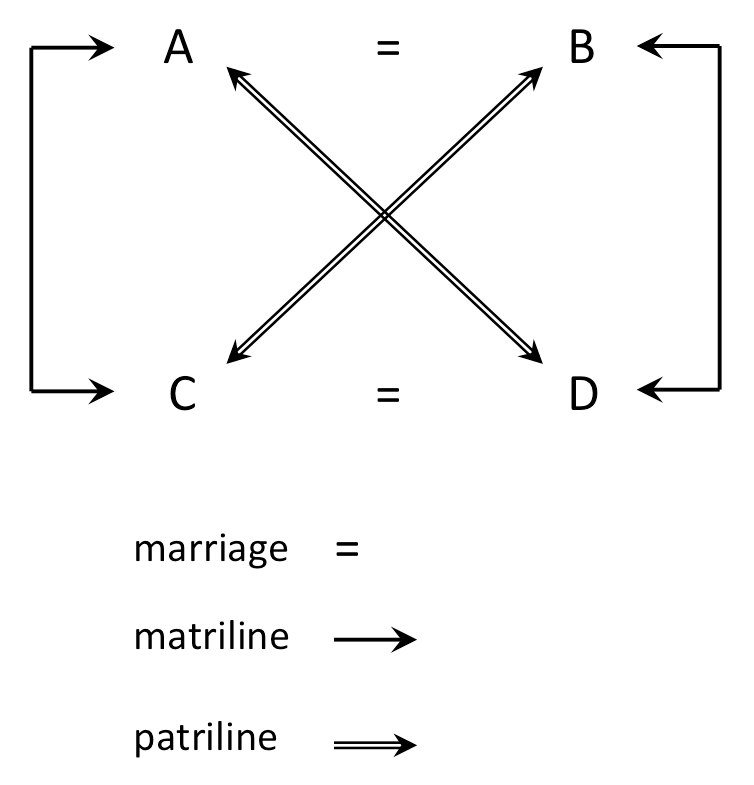
\includegraphics[width=0.5\textwidth,keepaspectratio]{figures/Fig05}
\caption{Sections (Northern Australia), from McConvell (1985:32), after 
Radcliffe-Brown (1931). }
\end{figure}







McConvell also describes the doubly complex subsection systems, in which 
the four categories of an erstwhile section system are each divided in 
two (see McConvell for diagram and discussion). There are structural 
consequences. For example, a cross-cousin is a possible wife in a 
section system, but not in a subsection system. 



This kind of system is widespread in Aboriginal Australia, shared by 
groups that have completely different languages. Evans (2012) likens the 
situation to that of the modern system of military ranks as officially 
standardized by the Geneva Convention: those groups who are members of 
the same culture area have direct translations for the same offices in 
the same system. In Northern Australia, a common cultural context has 
facilitated the widespread and stable nature of particular types of 
kinship systems and vocabularies. 



But there are many aspects of culture that seem more like items and less 
like systems. Eckert (2008) gives the example of a particular cut of 
jeans that happens to be fashionable among high school kids one year, 
though she urges us not to be tempted by the apparent individuability of 
such cultural elements. Something like the wearing of pegged pants or a 
way of pronouncing a certain vowel is always situated in an indexical 
field, as she puts it. When such things are borrowed or adopted into new 
social settings they may be \textquoteleft segmented' out from a historical and 
indexical constellation of signs and meanings. 



People who do this segmenting may know little of the larger (especially 
historical) connections, but they will nevertheless also give the item a 
place in a new system. Parry and Bloch (1989) make this point with 
reference to the historical adoption of money around the world: \textquoteleft in 
order to understand the way in which money is viewed it is vitally 
important to understand the cultural matrix into which it is 
incorporated' (Parry and Bloch 1989, 1).



Similarly, Sahlins (1999) says that when new elements-everything from 
money to snowmobiles-are incorporated into cultural contexts, they are 
adopted for local purposes and given a \textquoteleft structural position' in \textquoteleft the 
cultural totality' (Sahlins 1999). Sahlins celebrates the appropriation 
by neotraditional cultures/societies of elements from other societies 
(and note we can distinguish between processes of appropriation that 
alter the item so as to assimilate it into the receiving system versus 
those that alter the system so as to accommodate the incoming item; of 
course most of the time it is a combination of the two). 



Sahlins was critiquing the idea that cultures such as that of the Yupik 
are being contaminated by their borrowing of innovations associated with 
globalization. His point is that once borrowed, the items in question 
take on different meanings because of their new system context. 



\section{Are cultural totalities illusory?}


The kinds of systems and relations of incorporation in language and 
culture just discussed demonstrate that we are never dealing with 
detached cultural items. It does not follow, however, from the striking 
coherence of sub-systems like Australian sections and subsections that 
these ramp up into cultural totalities. It's possible that they do, and 
indeed the idea is supported by the fact that ethnographers have 
succeeded in writing reference descriptions of the knowledge, practices, 
values, and technologies of defined social/cultural groups (see e.g., 
Radcliffe-Brown 1922; Malinowski 1922; Firth 1936; Evans-Pritchard 1940; 
Fortes 1945, among many others). 



Similarly, linguists have succeeded in describing languages as 
totalities, not in the way a layperson might discretely label an 
imagined language (Dutch, Flemish, Serbian, Croatian, Thai, Lao, etc.), 
but rather in the technical sense of listing the lexicon and set of 
grammatical rules that any speaker will know. 



But what is our evidence that such totalities exist? Both the \textquoteleft whole 
systems' and the \textquoteleft parts' of language seem clearly identifiable at first 
glance, but both ideas crumble upon close inspection (Le Page and 
Tabouret-Keller 1985; Hudson 1996, inter alia). Any linguist knows that 
'a language'-in the sense of a community-wide system like French or 
Korean-is impossible to define extensionally, that is, by pointing at 
it: \textquoteleft as a totality it is inaccessible and indefinable; each of us has 
only partial experience of it' (Le Page and Tabouret-Keller 1985, 191). 



A language in the sense that we normally mean it constitutes a system 
insofar as it is a set of interrelated items, such as words, each of 
which appears to be a single unit or element. The system idea is 
especially clear in the case of language because, firstly, the set of 
interrelated items in a language is a large set, secondly, we have 
strong intuitions about what is part of language and what is not, and 
thirdly, this set contains multiple small or medium-sized sub-systems. 
But still we never encounter a language as such, only fragments of 
languages, items such as words and grammatical constructions, as 
instantiated in spoken utterances or in pieces of writing. 



In their masterpiece on the nature of language, Le Page and 
Tabouret-Keller (1985, 8-9) challenge us to face the problem of \textquoteleft how to 
know when to speak of separate systems': 



If we start from the concept of an underlying system this becomes an 
extremely difficult, if not insoluble, problem; if however we approach 
it from the point of view of the degree of coherence evidenced in the 
behaviour of a group of individuals, the problem is seen to be one of 
relationships and of stereotypes inherent in each individual. We do not 
ourselves then need to put a boundary around any group of speakers and 
say "\,These are speakers of Language A, different from Language B", 
except to the extent that the people think of themselves in that way, 
and identify with or distance themselves from others by their behaviour. 




Metalinguistic stances are real, but this does not mean that the systems 
they believe in are real in the same way. How, then, can we have a clear 
causal account of linguistic systems? The answer-to bring us back to the 
item/system problem-is in the causality of social behavior at the micro 
level.



\textit{to insert}: ‘The grammar of the closed system, and its predictions of ‘grammaticality’, become confused with the empirical judgements of people whose concept of ‘grammaticality’ - if they have one at all, which is in fact comparatively rare among the world’s population at large - is subsumed within a much wider concept of ‘acceptability’, a concept which takes account of creative, innovative, analogical, inventive and tolerant capacities of the human mind ignored by the closed systems of many grammarians.’ (Le Page and Tabouret-Keller:194)


